\documentclass[11pt]{article}
\usepackage[margin=1in]{geometry}
\usepackage{amsmath,amssymb,booktabs,graphicx,enumitem,hyperref,natbib,xcolor,array,tabularx,caption}
\usepackage[T1]{fontenc}
\usepackage{microtype}
\newcolumntype{L}{>{\raggedright\arraybackslash}X}
\newcolumntype{N}[1]{>{\raggedleft\arraybackslash}p{#1}}
\captionsetup[table]{font=small,labelfont=bf,justification=raggedright,singlelinecheck=false,skip=8pt}
\graphicspath{{figures/}}
\hypersetup{colorlinks=true,linkcolor=blue,citecolor=blue,urlcolor=blue}
\title{When Gene Ontology Evaluations Disagree: Identifiability-Aware Auditing and Remediation of Prediction Contracts}
\author{Anonymous Authors}
\date{}
\begin{document}
\maketitle
\begin{abstract}
Gene Ontology (GO) prediction scores depend on a contract combining model outputs, hierarchy processing, ontology and relation choices, eligibility rules, operating points, and evaluator semantics. A score discrepancy alone does not identify which choice caused it. We present a deterministic framework that replays available observations, enumerates exact and subset-minimal explanations within a registered candidate family, and plans a field-restricted action or abstains. An independently implemented matcher agreed with the production audit on all 336 retained controlled cases. In the 288-case primary suite, interaction candidates preserved 36 explanation sets missed by single-axis diagnosis; both methods agreed on the 48-case targeted extension. Restricting evidence to Fmax preserved only 236/288 and 12/48 explanation sets obtained under the original observation scope, respectively. Under one matched QuickGO/GO contract, our evaluator agreed with an externally authored CAFA-style implementation on all 594 endpoint-threshold rows within $10^{-12}$. Retrospective audits of four public model families exposed evaluator-absorbed closure, model-native hierarchy differences, incompatible operating points, and ontology mismatch. The remediation planner matched frozen specifications for 13 controlled and 3 real-artifact decisions. Counterfactual verification recovered all 6 recoverable controlled surfaces, while two retained real replay workflows reproduced 12/12 score exports and 1,188/1,188 threshold rows. These results support bounded contract diagnosis and restoration of evaluation comparability, rather than universal evaluator correctness or biological prediction improvement.
\end{abstract}

% The editor preview compiles this file as a standalone document. The section
% files under sections/ remain the modular source copies; their contents are
% inlined here so the built-in compiler can access the complete manuscript.

\section{Introduction}

Gene Ontology prediction is often summarized by a single F-measure or precision--recall curve. That summary hides a chain of semantic and operating-point decisions. A score matrix can be propagated through a model-native hierarchy, mapped to a different GO release, filtered by a namespace or term-universe rule, exported at a fixed threshold, and then evaluated by an implementation that performs its own ancestor propagation. Two scores can therefore disagree even when the underlying continuous predictions are identical. Conversely, an apparent model difference can disappear when the evaluation contracts are aligned.

This creates a practical problem for protein-function benchmarking: a discrepancy is observable, but its cause may not be identifiable. Existing CAFA evaluation and evaluator software define useful metric semantics \citep{radivojac2013cafa,jiang2016cafa,zhou2019cafa,piovesan2024cafaevaluator}; longitudinal evaluation and reporting frameworks improve reproducibility \citep{phan2026lafa,walsh2021dome,attafi2024domeregistry,garciavinuesa2026benchmarking}. Broader evaluation frameworks have also shown the value of coverage matrices, behavioral tests, composable evaluation modules, and explicit production-readiness checks \citep{liang2022helm,ribeiro2020checklist,goel2021robustnessgym,breck2017mltestscore}. Our focus is a complementary decision problem: which registered GO-contract changes are consistent with the available observations, and which corrective actions can be checked against a declared target?

We address this gap with a Gene Ontology evaluation-contract audit. A frozen contract records the score surface, ontology and relation set, hierarchy operators, eligibility and term universe, threshold representation, export policy, and evaluator semantics. Given a declared reference contract, an observed output and the available replay inputs, the audit searches a finite, registered explanation family. It reports what is identifiable under that observation scope without assuming access to the faulty source configuration. Figure~\ref{fig:workflow} shows how this diagnosis leads to a proposed action or abstention.

The paper makes four bounded contributions:
\begin{enumerate}[leftmargin=*]
\item an executable representation of GO evaluation contracts;
\item a bounded identifiability procedure based on exact and subset-minimal explanations, with explicit equivalence, unresolved and evidence-limited states;
\item a finite remediation library whose actions are selected from the diagnosis and verified over the complete target surface rather than by Fmax optimization; and
\item a model-output adapter registry that separates trusted format translation from scientific audit decisions and is demonstrated with four bounded real-format smoke witnesses.
\end{enumerate}

Our evidence is deliberately scoped. The primary controlled audit did not cover every attribution category, and a separate targeted extension tested the missing categories. Evaluator agreement was tested against one published CAFA-style implementation under a matched QuickGO/GO contract. Retrospective reconstruction covered four model families, two corpora, and two GO releases, while the remediation suite tested action safety within the frozen taxonomy and action library. These experiments assess evaluation comparability and contract restoration.

\begin{figure}[t]
\centering
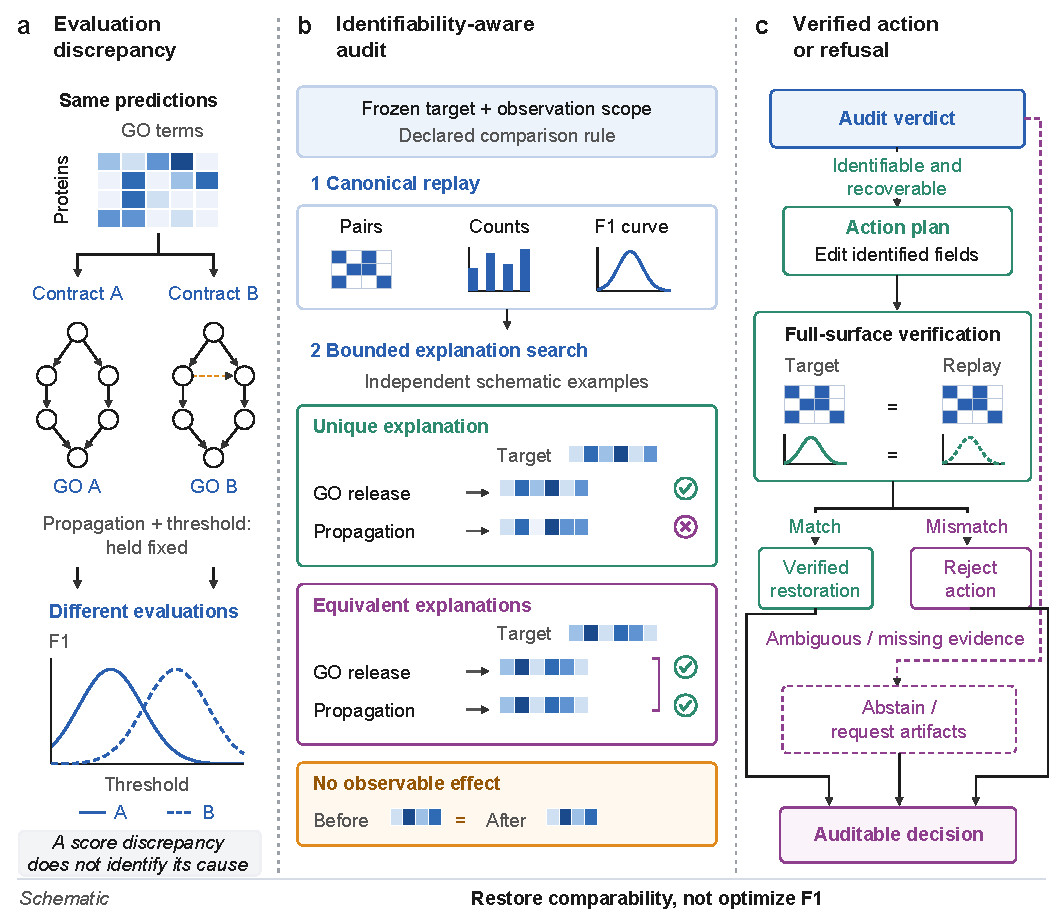
\includegraphics[width=\linewidth]{fig1_audit_revised.pdf}
\caption{Contract diagnosis and verification. (a) The same predictions can yield different evaluations under different GO contracts. (b) Candidate replay is compared with the available observation surface. The unique and equivalent explanations are separate schematic examples; check marks denote exact signature matches and crosses denote mismatches. An unchanged surface alone does not identify a hidden change. (c) The planner restricts proposed edits to diagnosed fields; acceptance requires target-surface verification. Ambiguous or insufficient evidence leads to abstention or a request for artifacts. Matrices and curves are schematic. The tested implementation combines counterfactual checks with two specific real replay workflows, rather than a general automatic patch executor.}
\label{fig:workflow}
\end{figure}

The remainder of the paper defines the contract and audit algorithm, presents controlled and real-pipeline evidence, and discusses the limits of retrospective contract attribution.

\section{Related work}

\paragraph{Community GO evaluation.}
The CAFA challenges established time-delayed evaluation of protein-function prediction and exposed the importance of ontology-aware precision and recall \citep{radivojac2013cafa,jiang2016cafa,zhou2019cafa}. The Gene Ontology resource itself is versioned and continuously maintained \citep{geneontology2021resource}. CAFA-evaluator provides a configurable implementation of DAG-aware prediction evaluation \citep{piovesan2024cafaevaluator}. Our work treats this evaluator layer as one component of a larger contract. We use an externally authored CAFA-style implementation as a matched reference, but do not claim official consortium equivalence or universal evaluator correctness.

\paragraph{Reproducible and longitudinal biological benchmarking.}
LAFA packages longitudinal annotation snapshots and containerized workflows for repeated assessment \citep{phan2026lafa}. DOME and the DOME Registry organize reporting requirements and community metadata \citep{walsh2021dome,attafi2024domeregistry}. Recent protein-ML benchmarking guidance also emphasizes persistent artifacts, interface contracts, provenance, and decision readiness \citep{garciavinuesa2026benchmarking}. These efforts motivate our contract representation and reproducibility records. The narrower contribution here is an executable GO-specific attribution layer that can return an equivalence class or refusal when the available artifacts do not identify a unique cause.

\paragraph{Multidimensional and behavioral evaluation.}
Several evaluation frameworks broaden model assessment beyond a single held-out score. HELM organizes scenarios and multiple desiderata, and reports both achieved coverage and dimensions that remain underrepresented \citep{liang2022helm}. CheckList turns behavioral capabilities into a matrix of test types and uses targeted cases to expose actionable failures \citep{ribeiro2020checklist}; Robustness Gym similarly separates datasets, transformations, metrics, and evaluation tasks into composable modules \citep{goel2021robustnessgym}. Production-oriented rubrics such as the ML Test Score make missing tests and monitoring requirements explicit \citep{breck2017mltestscore}. We adopt this coverage-first and action-oriented perspective, but specialize it to a different question: whether a discrepancy between two GO evaluations is identifiable from the artifacts that are actually observable. Our output is consequently a contract-level attribution or principled abstention, rather than a universal model score or a single readiness number.

\paragraph{Documentation and auditability.}
Model Cards and Datasheets make intended use, provenance, limitations, and known failure modes part of the reported scientific object \citep{mitchell2019modelcards,gebru2021datasheets}. We follow the same documentation principle for GO evaluation contracts, while making the recorded fields executable: source hashes, ontology snapshots, relation policies, score stages, operating-point rules, and evaluator semantics are replayed rather than merely described. This distinction lets the audit verify a proposed remediation on the full observation surface and preserve a non-estimable verdict when required evidence is absent.

\paragraph{Hierarchy-aware prediction.}
Hierarchical multi-label predictors enforce consistency during model training or inference, for example through structured losses, hierarchical ensembles, or true-path rules \citep{barutcuoglu2006hierarchical,schietgat2010hierarchical,valentini2011truepath,giunchiglia2020coherent}. These are model-side mechanisms. Our audit instead separates model-native hierarchy processing from evaluator-side ancestor propagation and evaluation-time GO topology. This distinction matters because an explicit portable closure can be metric-inert when the downstream evaluator performs the same propagation.

\paragraph{Testing and diagnosis.}
Software-testing literature studies oracle limitations, formal specifications, differential testing, and conformance testing \citep{barr2015oracle,hierons2009formaltesting}. Model-based diagnosis provides a foundation for relating system descriptions and observations to minimal diagnoses \citep{reiter1987diagnosis}. We do not introduce general minimal diagnosis. Our implementation enumerates a registered family of concrete GO-contract edits and compares their replayed outputs under explicitly limited observations. Its contribution lies in the GO contract semantics, evidence-dependent verdicts and target-restoration workflow, rather than a new general diagnosis theory.

\paragraph{Public model pipelines.}
InterLabelGO+, SPROF-GO, DeepFRI, and ProtNote represent heterogeneous protein-function prediction output styles \citep{liu2024interlabelgo,yuan2023sprofgo,gligorijevic2021deepfri,char2025protnote}. The purpose of using these systems is not to rank predictors or claim that one model is better. They provide realistic output contracts: native matrices, logits requiring a sigmoid transform, sparse threshold exports, and mixed hierarchy conventions. The audit makes those choices visible before comparing metrics.

\section{Methods}

\subsection{Evaluation contract}
Let $P$ be the protein universe, $T$ the GO term universe, and $S:P\times T\to[0,1]$ the continuous score surface. A contract $C$ records the ontology snapshot $G$ and relation set $R$, alternative and obsolete-term policies, prediction and truth propagation operators, eligibility and averaging rules, threshold grid and comparison boundary, score representation, export policy, and evaluator semantics. It also records source and input hashes. Table~\ref{tab:contract-axes} lists the required evidence. Model-output reconstruction uses no outcome labels; metric computation, truth propagation and explicitly label-dependent universe rules require the declared annotations. Private injected-fault labels and expected diagnoses are excluded from diagnostic inputs.

\begin{table}[tbp]
\centering
\small
\setlength{\tabcolsep}{5pt}
\renewcommand{\arraystretch}{1.18}
\caption{Observable evidence required to specify an evaluation contract.}
\label{tab:contract-axes}
\begin{tabularx}{\linewidth}{@{}>{\hsize=.65\hsize}L>{\hsize=1.15\hsize}L>{\hsize=1.2\hsize}L@{}}
\toprule
Contract component & Required evidence & Comparison risk if absent \\
\midrule
Score stage & Continuous scores, protein and term order, export rule & Hidden processing stages cannot be reconstructed. \\
\addlinespace[3pt]
Native hierarchy & Relation matrix, processing code, asset version & Native processing may be confused with current GO. \\
\addlinespace[3pt]
Ontology & GO snapshot, relation set, obsolete and alternative-ID policies & Residual differences cannot be assigned to version changes alone. \\
\addlinespace[3pt]
Operating point & Threshold grid, boundary rule, rounding, export filters & Fixed-threshold F and Fmax are not directly comparable. \\
\addlinespace[3pt]
Eligible universe & Protein and term inclusion rules & Different denominators may resemble model-quality differences. \\
\addlinespace[3pt]
Evaluator & Propagation, averaging, root and normalization rules & Evaluation choices may resemble method improvements. \\
\bottomrule
\end{tabularx}
\end{table}

We distinguish the model-native score surface from portable evaluation transformations. For a threshold $\tau$, the evaluator consumes a set-valued prediction surface $\Pi_C(S,\tau)$ and truth surface $\Gamma_C(Y)$. The reported curve is
\[
  M_C(\tau)=\operatorname{Eval}_C(\Pi_C(S,\tau),\Gamma_C(Y)),
\]
where $M_C(\tau)$ contains the declared metric outputs and $F_C(\tau)$ denotes its protein-centric F1 component. Then $F_{\max}(C)=\max_{\tau\in\mathcal{T}}F_C(\tau)$. This maximum describes a frozen contract; it is never used to choose a repair action.

\subsection{Bounded identifiability}
Let $\Omega$ denote the registered contract axes and $\mathcal{A}\subseteq 2^\Omega$ the explicitly registered family of candidate edits. Each $A\in\mathcal{A}$ selects fixed alternative field values, applied jointly to a declared baseline contract before replay. Let $O$ be the observed output to explain and $\pi_L$ its available evidence projection. The explanation set is
\[
  E(O)=\{A\in\mathcal{A}: \pi_L(\operatorname{Replay}(C;A))=O\}.
\]
The subset-minimal explanations are $E_{\min}(O)=\{A\in E(O):\nexists A'\in E(O),\ A'\subsetneq A\}$. Minimality is relative to the registered family, not a search over every possible edit or a global action-cost optimum. One nonempty minimal set can contain several axes. Several incomparable minimal sets form an equivalence class; no match leaves the discrepancy unresolved. If the empty set matches, the baseline is observationally equivalent to the supplied output.

The controlled registry contains 20 candidates: the empty set, 11 single-axis edits and eight specified two-axis interactions. The axes concern prediction and truth closure, relation set, namespace and root policies, term universe and its label dependence, threshold comparison and representation, alternative IDs and obsolete IDs. Supplementary Methods S1--S2 specify their fixed forward semantics, operation order and registered pairs. These are candidate explanations of an observed discrepancy; corrective edits subsequently restore the corresponding fields to a separately frozen target contract.

The pairwise projection retains protein--term predictions and truth together with counts and metric curves. Counts-only evidence removes pair identities; aggregate-only evidence additionally removes per-protein counts. Candidates are projected to exactly the channels available in the observed output. Synthetic matching uses exact typed structural equality: mapping order is immaterial, sequence order is retained, and floating values retain their binary representation, including signed zero. This rule is distinct from the $10^{-12}$ tolerance used for external evaluator agreement. Aggregate-only evidence does not authorize a specific pairwise diagnosis, even when the registered family has one nonempty minimal match. Counts-only and pairwise evidence can support a unique explanation within their declared scope. Masking and no-effect labels in controlled scoring additionally use private intervention records; they are not inferred from public signatures alone. Evaluator absorption requires separate replay evidence.

\subsection{Audit and remediation algorithm}
The audit proceeds in five stages: (i) extract and hash the declared contract; (ii) replay a canonical reference surface; (iii) enumerate candidate explanations and compare their observable signatures; (iv) assign an identifiability verdict and identify missing artifacts; and (v) plan an action from a finite library. The action library contains no action, apply a patch, remove redundancy, recompute, request re-export, do not compare, and abstain.

The matching procedure is explicit: replay each registered candidate; retain those equal to the observed projection; discard any matching set with a matching strict subset; and return the remaining sets with the evidence-dependent verdict. No case identifier, injected-fault label or expected diagnosis enters these steps. Missing inputs are reported before a claim requiring them is made. Subset filtering needs at most quadratically many candidate-pair comparisons after replay; forward computation and observation comparison are separate costs.

A patch recommendation requires one supported nonempty minimal explanation, the required replay inputs, a target contract frozen before diagnosis, and edits confined to the identified fields. This is a registered-field restriction, not a global minimum-cost guarantee. Removing redundancy is appropriate when a transformation is absorbed by the evaluator. Recomputation aligns retained continuous scores under the target contract. Missing continuous scores can require re-export; incompatible operating points can require refusing comparison; ambiguity requires abstention. Acceptance checks all channels declared by the target, rather than Fmax alone. Controlled restoration uses precomputed counterfactual surfaces. Real restoration is tested in two specific replay workflows; a general interpreter that executes arbitrary emitted patches is not evaluated.

\subsection{Validation design}
The primary controlled audit and targeted extension separate public observations from private injection records. A subsequent regression check revisits all 288 and 48 retained cases with an independent reference matcher. The reference compares typed structures directly and constructs a cardinality-ordered antichain; it imports neither production enumeration nor signature functions. Twelve hand-specified boundary checks and seven representation checks precede the regression. This independently checks matching, minimality, equivalence partitions and public verdicts. Candidate surfaces still use the existing forward implementations; their common projection and metric code is not an independent evaluator.

For the same cases and available evidence, we compare single-axis diagnosis (empty plus 11 singleton candidates), full diagnosis (20 candidates), and an information ablation retaining only Fmax over the original six thresholds. Explanation-set preservation means exact agreement with the independent reference under the original observation scope. Unique-diagnosis coverage uses the public verdict rule, separately from historical injected-category denominators. Method outputs are sealed before comparison with reference outcomes. Metadata inspection with target recomputation is also assessed for feasibility, but the public cases do not disclose the actual faulty source contract; its attribution performance is therefore not estimable. Related observation variants are not treated as independent samples for significance testing.

The matched evaluator comparison uses six real endpoint matrices, one QuickGO cohort, one GO snapshot, and 99 thresholds. The retrospective audits reconstruct specified retained transforms for four public model families; two branches require rerunning the models. Ontology mismatch compares native relation reachability with the evaluation-time GO graph. The remediation suite assesses frozen-rule conformance, controlled counterfactual restoration and retained real replay separately. Supplementary Table S4 summarizes the validation questions and their evidence boundaries.

\subsection{Extensible adapters}
The audit core consumes a canonical continuous-score interface. The registry has six built-in adapters: canonical delimited text, generic HDF5 matrices, two verified HDF5 aliases, DeepFRI JSON, and ProtNote logits. Third-party adapters register explicitly through trusted local Python code. The interface receives an input path, output directory, and declared options; it does not receive truth, metric APIs, threshold-selection APIs, or remediation authority. Users must declare the output stage and score semantics. Real-format evidence is bounded to four witnesses: InterLabelGO+ MFO (568$\times$1,571), SPROF-GO MFO (568$\times$790), DeepFRI MF (11,202$\times$489), and an 8$\times$16 ProtNote frozen-HDF slice. The current storage authority supports a 91.30\% byte reduction for one InterLabelGO+ MFO witness, not a universal compression or semantic-equivalence claim.

\section{Results}

\subsection{Controlled identifiability and honest coverage}
The primary controlled audit retained 288 cases: 192 with protein--term pair observations, 48 with counts only, and 48 with aggregate metrics only. Reconstruction, masking, no-effect classification, unknown-case handling, false-gain detection, and reduced-observability checks met their specified criteria. Reconstruction produced no signature mismatches or metric errors. In the 96 eligible unique-attribution cases, exact recovery of the subset-minimal explanation sets was 100\%. However, namespace policy, term-universe selection, and label-dependent term-universe selection had no positive identifiable examples, and no case was eligible for the equivalence-class test. Overall attribution coverage therefore remained not estimable (Supplementary Table S3); accuracy on the observed cases did not establish coverage of the missing categories. Figure~\ref{fig:coverage} summarizes this coverage-first result, while Supplementary Table S3 reports the exact assessment-specific denominators.

A separate targeted extension tested 48 additional cases, including 24 eligible for unique attribution and eight for equivalence-class assessment. Precision and recall for the targeted discrepancy types and complete equivalence-class coverage were all 100\%. These historical recovery rates measure agreement with synthetic fixture expectations, some of which shared the auditor's enumeration routine. The independent regression below checks that routine separately without changing the original coverage categories or denominators. The extension supplements the primary audit without changing its recorded coverage limitation.



\begin{figure}[t]
\centering
\IfFileExists{fig2_identifiability_coverage.pdf}{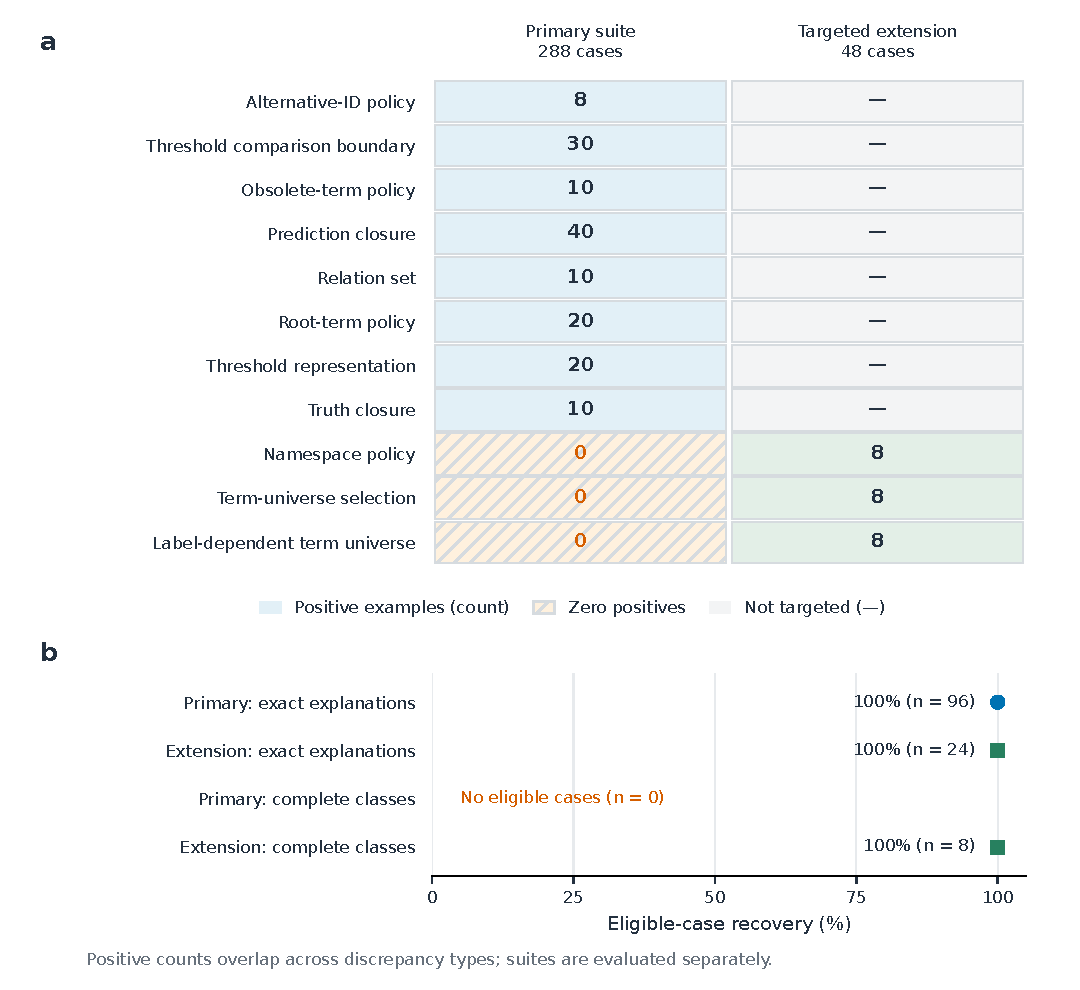
\includegraphics[width=\linewidth]{fig2_identifiability_coverage.pdf}}{\fbox{\parbox{0.92\linewidth}{Figure 2 source: \texttt{fig2\_identifiability\_coverage.svg}.}}}
\caption{Positive-example coverage and eligible-case recovery in two separately evaluated controlled suites. (a) Counts of positive examples for each discrepancy type in the primary suite (288 cases) and targeted extension (48 cases). Hatched zeros indicate no positive examples; dashes indicate types not targeted in the extension. A case may contribute positive examples to more than one discrepancy type. (b) Exact recovery of subset-minimal explanation sets and complete equivalence-class recovery, with assessment-specific denominators. ``No eligible cases'' denotes a zero denominator and therefore a not-estimable assessment; it is not zero accuracy. Positive counts are not performance scores: precision and recall were 100\% for each type with positive examples. The extension supplies targeted coverage without changing the primary suite's recorded limitations.}
\label{fig:coverage}
\end{figure}

\subsection{Independent verification and diagnostic information}
The independent matcher agreed with both newly computed production outputs and sealed historical public outputs in all 336 cases, including exact candidates, minimal explanation sets, equivalence partitions and public states. All 12 boundary checks and seven representation checks passed. The existing forward implementations agreed on 1,440 candidate surfaces; all 112 evidence-reduction checks and 32 comparisons with previously hand-specified expectations passed. The regression took 864.4 seconds with a peak resident memory of 702 MiB on the local CPU environment; no GPU was used. This is a regression on retained cases, not a new blind sample or a new independent ontology evaluator.

Table~\ref{tab:diagnostic-comparison} separates candidate-family coverage from observation loss. In the primary suite, all 36 explanation sets missed by single-axis diagnosis required registered multi-axis interactions. Of these, 30 admitted unique diagnosis under the public evidence rule: 24 pairwise and six counts-only cases. In the targeted extension, single-axis and full diagnosis preserved the same sets. Neither method made an unsupported unique assertion in either suite. Field-rule checks found no violations among 134 single-axis and 164 full-diagnosis patch recommendations in the primary suite. The extension lacked the complete target contract required for this action assessment, so its action result is not estimable.

\begin{table}[tbp]
\centering
\small
\setlength{\tabcolsep}{5pt}
\renewcommand{\arraystretch}{1.16}
\caption{Explanation-set preservation and unique-diagnosis coverage on the retained controlled cases.}
\label{tab:diagnostic-comparison}
\begin{tabularx}{\linewidth}{@{}L N{0.18\linewidth} N{0.18\linewidth} N{0.21\linewidth}@{}}
\toprule
Method & Candidate count & Sets preserved & Correct unique diagnoses \\
\midrule
\multicolumn{4}{@{}l}{\textit{Primary suite: 288 cases}} \\
Single-axis & 12 & 252/288 & 134/164 \\
Full diagnosis & 20 & 288/288 & 164/164 \\
Fmax-only ablation & 20 & 236/288 & --- \\
\midrule
\multicolumn{4}{@{}l}{\textit{Targeted extension: 48 cases}} \\
Single-axis & 12 & 48/48 & 30/30 \\
Full diagnosis & 20 & 48/48 & 30/30 \\
Fmax-only ablation & 20 & 12/48 & --- \\
\bottomrule
\end{tabularx}
\par\smallskip
{\footnotesize\raggedright Sets are compared with the independent reference at each case's original observation scope. The unique-diagnosis denominators use public evidence eligibility and do not replace the historical category denominators in Supplementary Table S3. Dashes denote unique attribution disallowed by the aggregate-evidence policy, not an additional empirical failure. No method receives private injected-fault labels.\par}
\end{table}

Fmax-only evidence preserved 236/288 and 12/48 original explanation sets. This measures information lost by projection, not an error in its matching algorithm. Its absence of unique-diagnosis outputs follows the aggregate-evidence refusal rule and is not itself evidence of information loss. On the primary suite, production matching took 728.9 seconds with the full family and 443.2 seconds with single-axis candidates in separate runs on the same machine; these are unoptimized implementation timings. Metadata inspection could not be scored for attribution because the faulty source configuration was not public. We therefore make no superiority claim over configuration inspection with complete metadata.

\subsection{Agreement with a matched external evaluator}
The external comparison used BioComputingUP/CAFA-evaluator 1.3.0 at a locked source revision recorded in the evidence ledger. On one QuickGO cohort and one GO snapshot, six endpoints were evaluated at 99 thresholds. All 594 rows were present in both implementations. Integer counts matched exactly, no metric difference exceeded $10^{-12}$, and the maximum absolute floating error was $3.33\times10^{-16}$. Table~\ref{tab:evaluator-agreement} also reports matched comparisons for the retained model outputs. Agreement is limited to the tested contracts and does not establish official CAFA equivalence or correctness under all evaluator settings.

\begin{table}[tbp]
\centering
\small
\setlength{\tabcolsep}{5pt}
\renewcommand{\arraystretch}{1.18}
\caption{Agreement with the external evaluator under matched contracts.}
\label{tab:evaluator-agreement}
\begin{tabularx}{\linewidth}{@{}L N{0.12\linewidth} N{0.19\linewidth} N{0.20\linewidth}@{}}
\toprule
Comparison & Curves & Matched rows & Max.\ absolute error \\
\midrule
Matched-snapshot evaluation & 6 & 594/594 & $3.33\times10^{-16}$ \\
\addlinespace[3pt]
InterLabelGO+ / SPROF-GO retained stages & 27 & 2,673/2,673 & $3.33\times10^{-16}$ \\
\addlinespace[3pt]
ProtNote / DeepFRI retained outputs & 6 & 594/594 & $3.33\times10^{-16}$ \\
\bottomrule
\end{tabularx}
\par\smallskip
{\footnotesize\raggedright Each curve contains 99 thresholds. The 27 retained-stage curves do not represent 27 independent models. The floating-point comparison tolerance is $10^{-12}$.\par}
\end{table}

\subsection{Four-family retrospective reconstruction}
The first real-pipeline batch covered InterLabelGO+ and SPROF-GO on 568 proteins and a frozen GO 2026-07-26 snapshot; the second covered ProtNote and DeepFRI on 11,202 proteins and a frozen GO 2025-06-01 snapshot. Each batch included biological process (BP), cellular component (CC), and molecular function (MF). The first audit reconstructed specified retained output transforms and evaluated 2,673 curve rows with the matched evaluator. The two unobserved branches, InterLabelGO+ DIAMOND hybrid and SPROF-GO label diffusion, remained not assessable without a rerun. The second audit reconstructed six retained ProtNote/DeepFRI endpoints under the locked replay protocol and matched 594/594 threshold rows. Figure~\ref{fig:families} summarizes the declared stages, frozen snapshots, and explicitly unassessed branches. These are retrospective pipeline audits, not unseen or prospective biological validation.

\begin{figure}[t]
\centering
\IfFileExists{fig3_four_family_pipeline_map.pdf}{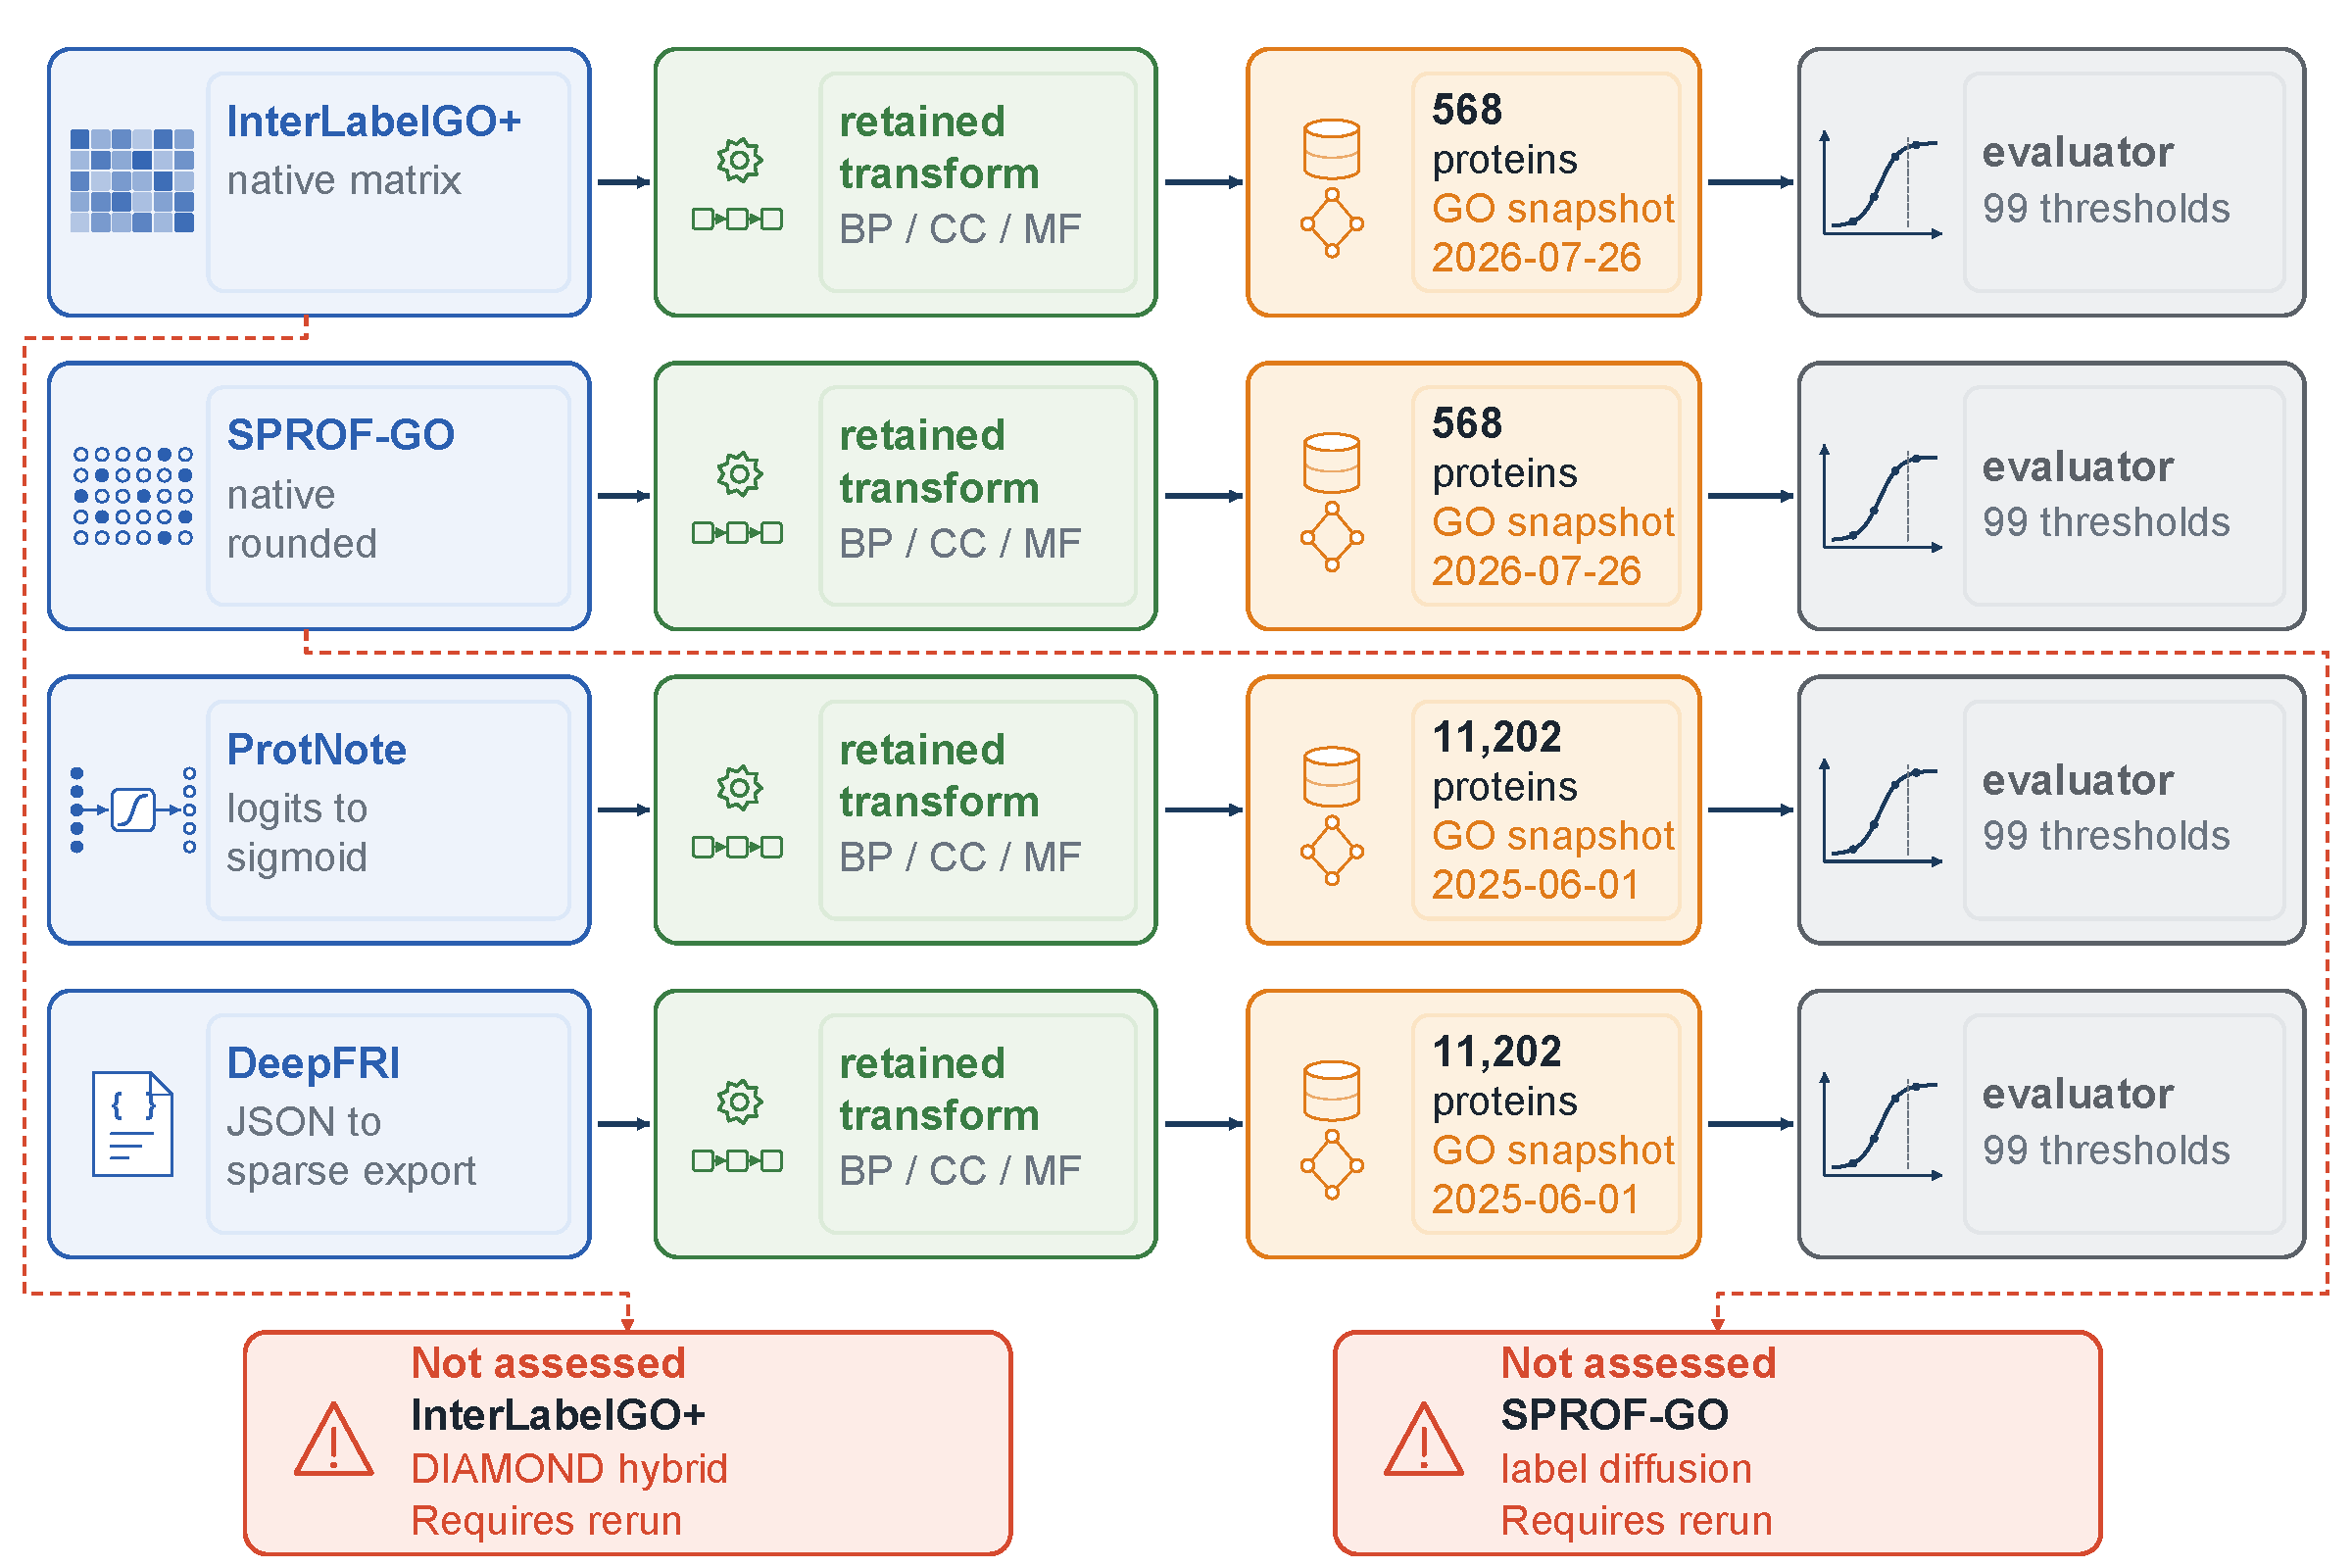
\includegraphics[width=\linewidth]{fig3_four_family_pipeline_map.pdf}}{\fbox{\parbox{0.92\linewidth}{Figure 3 source: \texttt{fig3\_four\_family\_pipeline\_map.svg}.}}}
\caption{Coverage map for retrospective contract replay across four public model families. The diagram records declared output stages, frozen protein and ontology snapshots, and the two released branches that remain unassessed without rerunning the models. Dashed connectors associate each unassessed branch with its model family. Matrix patterns and miniature curves are schematic illustrations, not measured outputs; this is not a performance ranking.}
\label{fig:families}
\end{figure}

\subsection{Hierarchy processing and ontology mismatch}
In the retained-transform audit, portable current-GO ancestor max was metric-inert at all six endpoints because the matched evaluator already propagated ancestors. The correct interpretation is evaluator absorption, which supports removing redundant propagation; it is not evidence for hierarchy irrelevance or model improvement. Native residuals were non-positive in all six endpoints and strictly negative in five.

The ontology mismatch audit localized structural differences between native matrices and the current GO graph. Relation-set Jaccard values ranged from 0.425 to 0.972, while retained current-GO violation counts ranged from 2,496 to 82,543 (Figure~\ref{fig:mismatch}). The association analysis related mismatch burden (unsupported-pair rate plus missing-pair rate) to contract-residual Fmax across only six endpoints: Pearson $r=0.1185$, Spearman $\rho=-0.7143$, and no generalization p-value. This is descriptive localization, not evidence for a predictive or causal relationship; the figure is used to show structural heterogeneity, not to fit a performance law.

\begin{figure}[t]
\centering
\IfFileExists{fig4_ontology_mismatch.pdf}{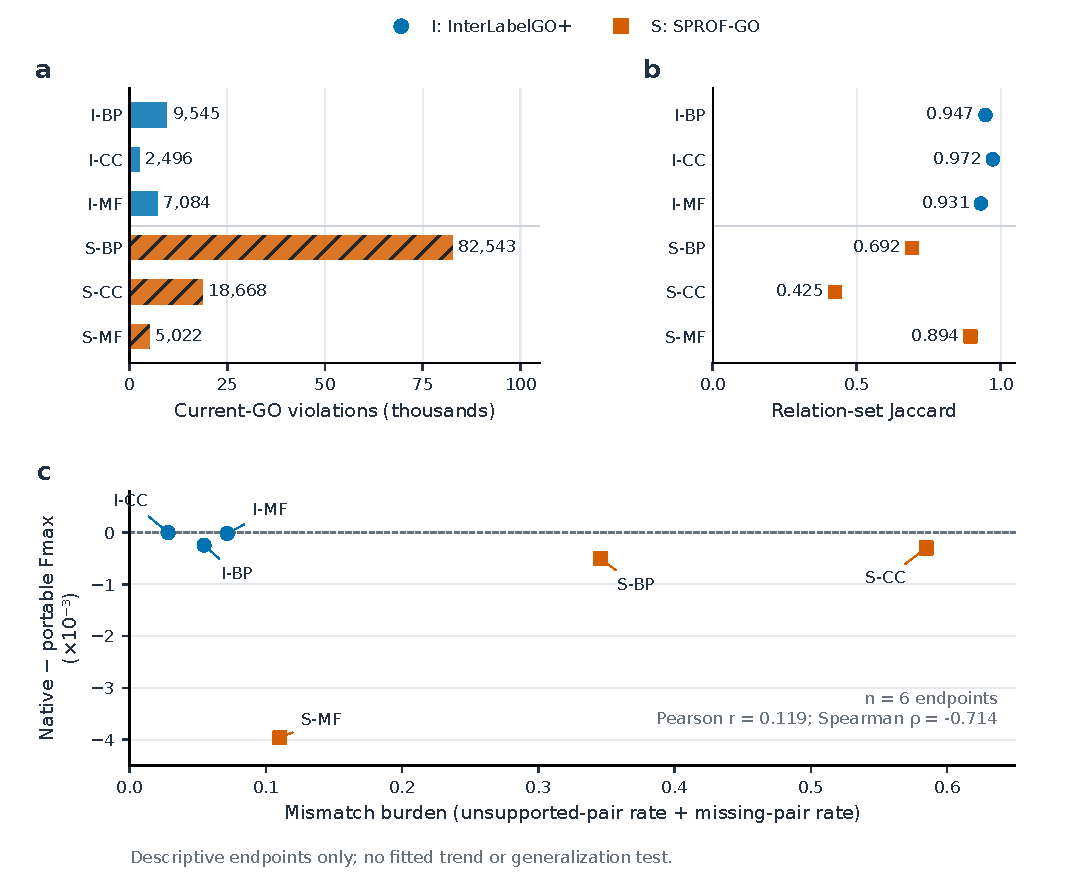
\includegraphics[width=\linewidth]{fig4_ontology_mismatch.pdf}}{\fbox{\parbox{0.92\linewidth}{Figure 4 source: \texttt{fig4\_ontology\_mismatch.svg}.}}}
\caption{Structural mismatch and contract residuals for six frozen model--namespace endpoints. (a) Retained current-GO violation counts; bar labels give exact counts and the axis is in thousands. These absolute counts are not normalized across endpoints. (b) Native/current relation-set Jaccard values. (c) Mismatch burden (unsupported-pair rate plus missing-pair rate) versus native minus portable Fmax, in units of $10^{-3}$. I and S denote InterLabelGO+ and SPROF-GO; BP, CC and MF denote GO namespaces. The six endpoints share a 568-protein cohort and frozen GO 2026-07-26 snapshot. The endpoints represent two model families across three namespaces, not independent replicates. Correlations describe these endpoints only, with no fitted trend, generalization test or causal claim.}
\label{fig:mismatch}
\end{figure}

\subsection{Actionability and remediation safety}
The remediation suite contained 13 controlled decisions and three preregistered real-artifact decisions. All 16 decisions matched the frozen action specification. Six controlled surfaces were recoverable in the precomputed counterfactual library and all six were restored. The recorded safety checks found zero false repairs, zero non-minimal repairs under the registered-field rule, and zero metric-optimized actions. These counts assess specification conformance, not independently labeled real-world action correctness. In real counterfactual replay, two specific workflows each reproduced 6/6 score exports and 594/594 threshold rows, totaling 12/12 exports and 1,188/1,188 curve rows (Figure~\ref{fig:remediation}). Table~\ref{tab:remediation-safety} separates action agreement from restoration. The associated Fmax changes are contract-alignment quantities, not model improvements.

The ontology-alignment case illustrates the user-facing decision. The inputs are retained pre-hierarchy scores, native relations, annotations and a frozen target GO contract. Relation comparison identifies a structural discrepancy without assuming a direction of performance change. When the required scores are available, the workflow recomputes propagation and evaluation under the target contract, then compares score exports and the complete curve against the target. The retained record reports six matching exports and 594 restored rows. Without pre-hierarchy scores, the report must request an appropriate export or retain an unresolved restoration limit. Our later reconciliation of the three case narratives used retained summaries; it did not rerun these real workflows.

\begin{table}[tbp]
\centering
\small
\setlength{\tabcolsep}{5pt}
\renewcommand{\arraystretch}{1.18}
\caption{Action selection, restoration and safety in the remediation suite.}
\label{tab:remediation-safety}
\begin{tabularx}{\linewidth}{@{}>{\hsize=1.3\hsize}L N{0.18\linewidth}>{\hsize=.7\hsize}L@{}}
\toprule
Assessment & Result & Unit \\
\midrule
Controlled action selection & 13/13 & Specification matches \\
Real-artifact action selection & 3/3 & Specification matches \\
Recoverable controlled surfaces & 6/6 & Restored surfaces \\
Real score exports & 12/12 & Reproduced exports \\
Real threshold evaluations & 1,188/1,188 & Reproduced rows \\
\midrule
False repairs & 0 & Actions \\
Non-minimal repairs & 0 & Actions \\
Metric-optimized actions & 0 & Actions \\
\bottomrule
\end{tabularx}
\par\smallskip
{\footnotesize\raggedright Success means agreement with the frozen action specification or restoration of the complete target surface. These counts do not measure biological prediction improvement.\par}
\end{table}

\begin{figure}[t]
\centering
\IfFileExists{fig5_remediation_verification.pdf}{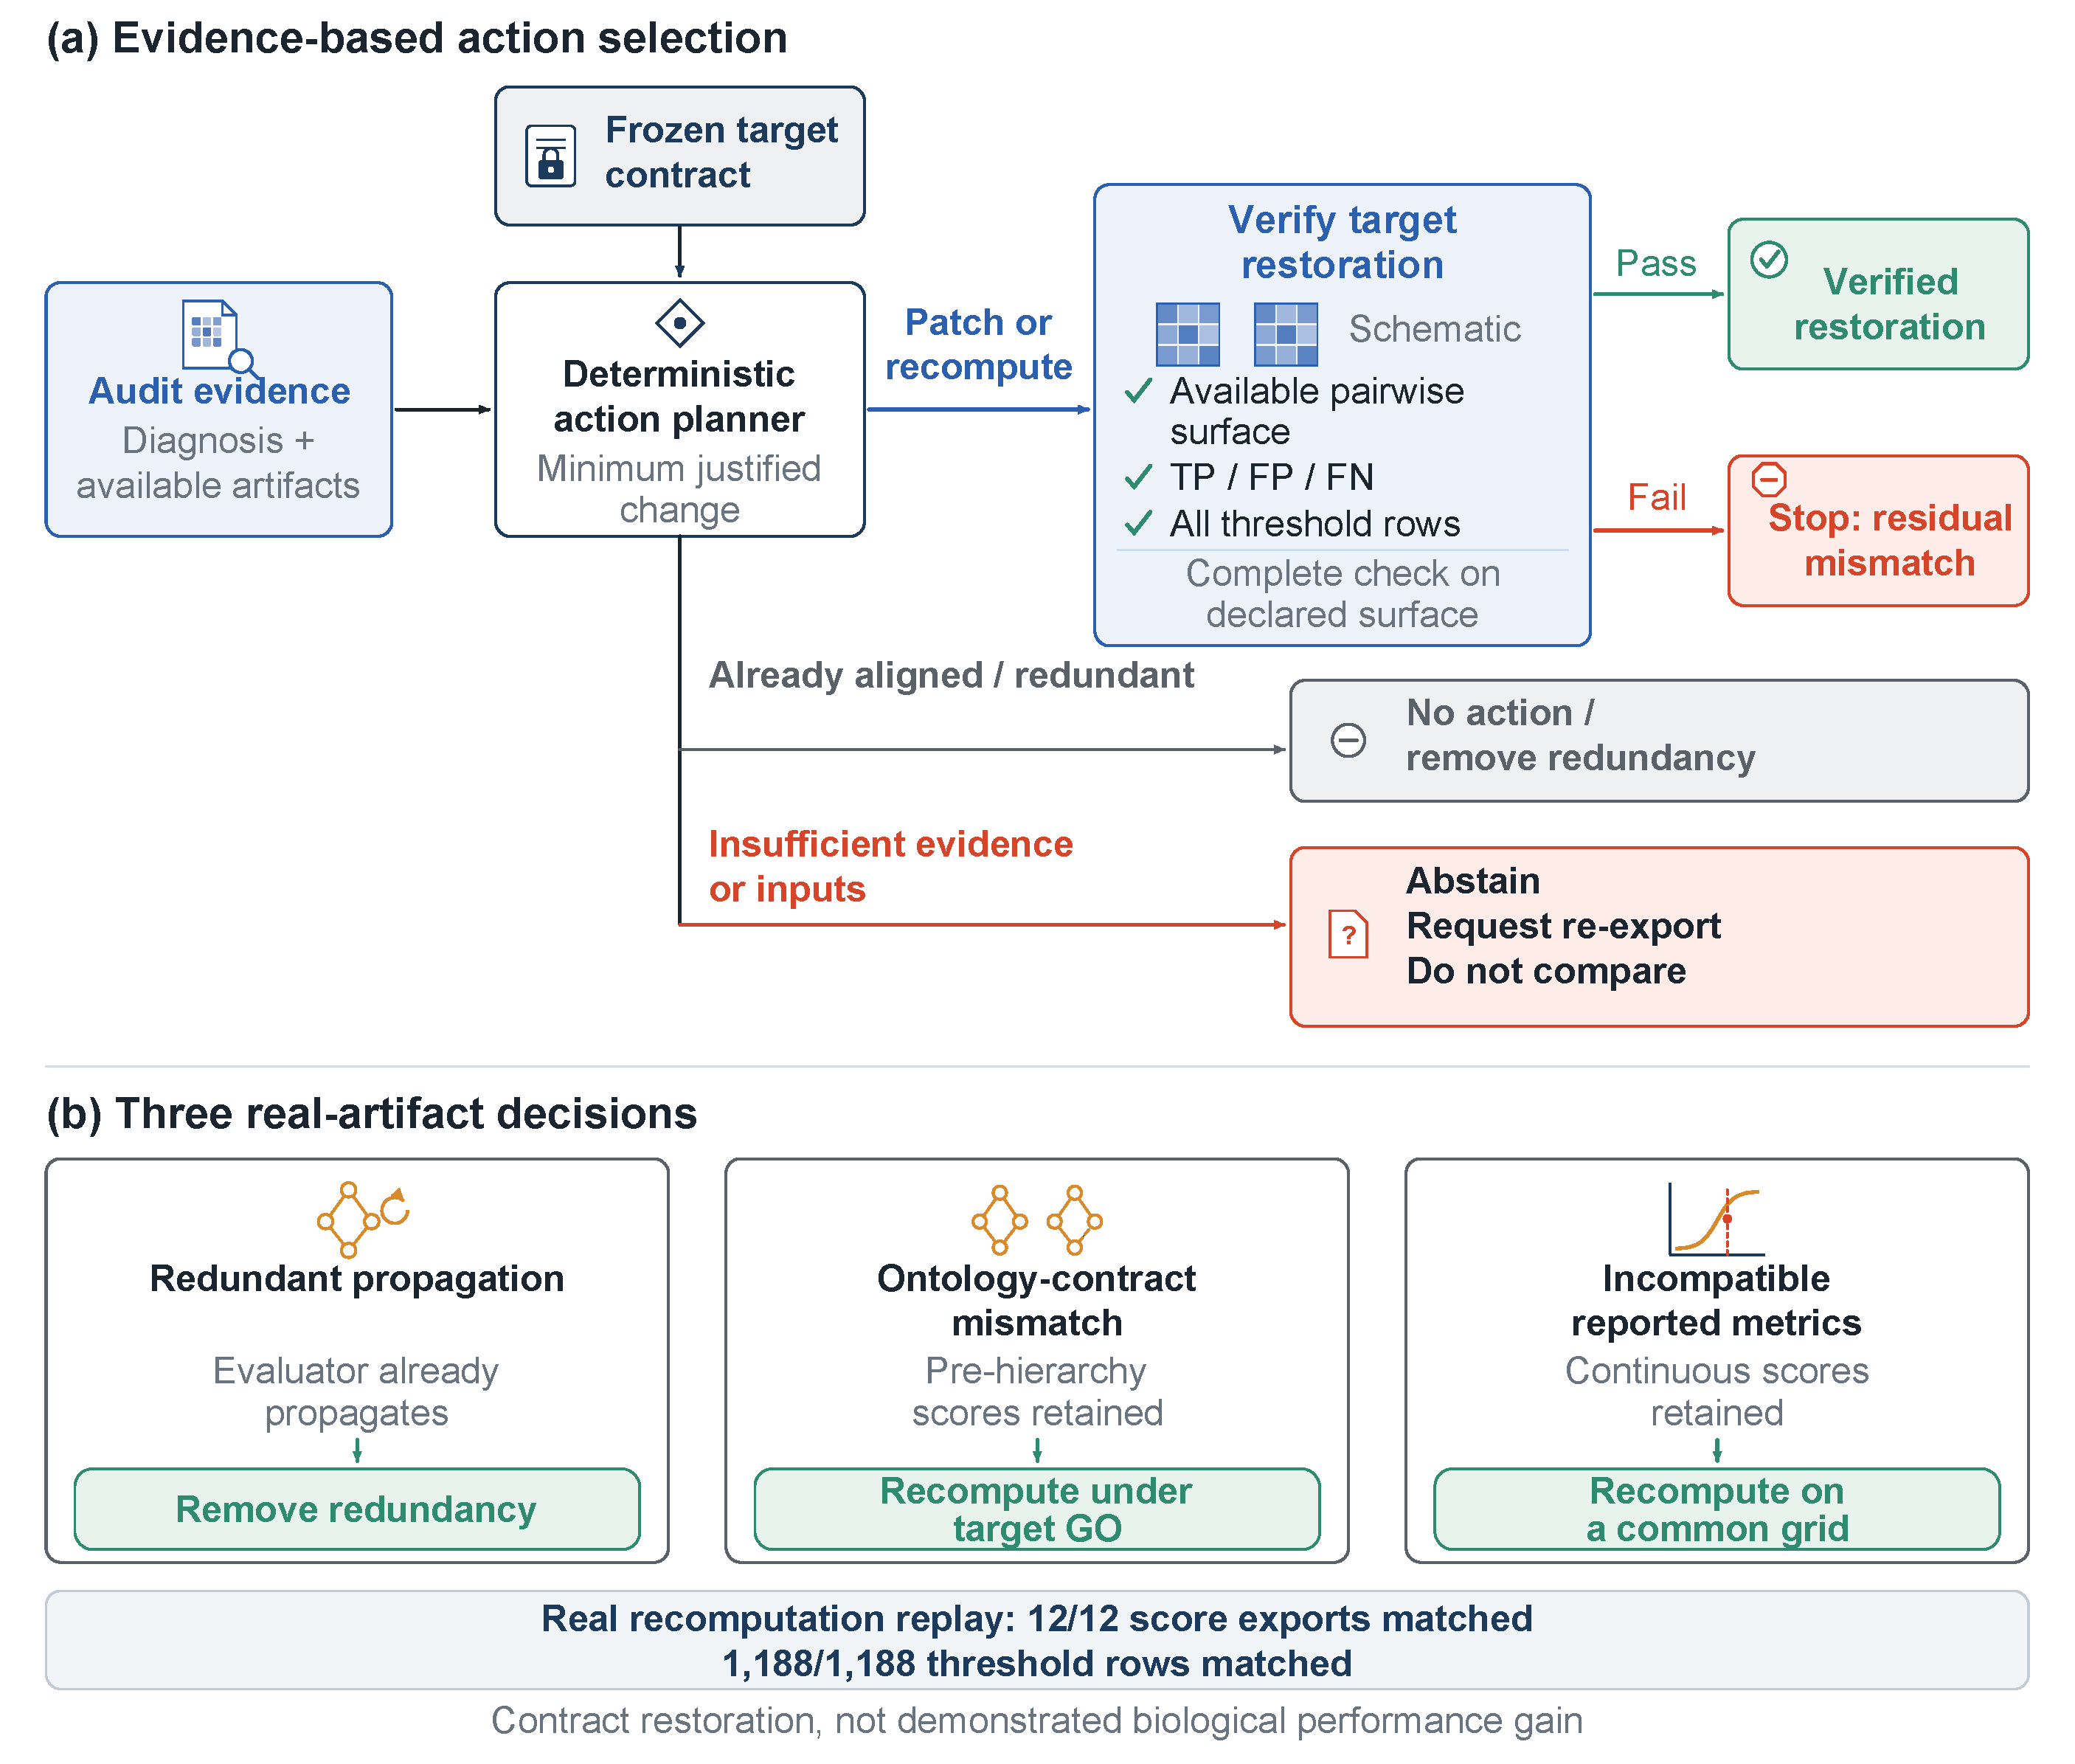
\includegraphics[width=\linewidth]{fig5_remediation_verification.pdf}}{\fbox{\parbox{0.92\linewidth}{Figure 5 source: \texttt{fig5\_remediation\_verification.svg}.}}}
\caption{Evidence-based remediation selects an action from a frozen library and verifies target-contract restoration when reconstruction is supported. (a) A deterministic planner combines bounded diagnosis, available artifacts and a frozen target contract. Patch or recomputation outcomes require complete verification on the declared observation surface; residual discrepancies stop acceptance. Already aligned or redundant processing and cases requiring abstention, re-export or refusal of comparison follow separate routes. (b) Three real-artifact decisions illustrate redundancy removal and recomputation from retained continuous scores. The separate real-replay validation reproduced 12/12 score exports and 1,188/1,188 threshold rows. Miniature graphs, matrices and curves are schematic. These results establish contract restoration within the tested scope, not biological prediction improvement.}
\label{fig:remediation}
\end{figure}

\subsection{Adapter portability and reproducibility}
The adapter registry implements six built-in adapters and explicit trusted-plugin registration. The four real-format smoke witnesses are dimensioned in Methods; the ProtNote witness is explicitly an 8$\times$16 slice. One InterLabelGO+ MFO witness decreased storage from 36,716,347-byte long TSV to 3,195,857-byte compressed HDF5, a 91.30\% byte reduction. The compact storage authority does not independently establish full semantic equivalence or complete direct-HDF5 audit equivalence, so neither is claimed here. Archived reproduction reports record matching scientific outputs for 87 artifacts in the first pipeline audit and nine in the ontology mismatch audit under their declared exclusions. We additionally reconciled these reports against frozen locks, retained manifests and locally available artifact bytes; this reconciliation did not rerun the scientific pipelines.

A separate diagnosis-component capsule contains three retained examples covering a unique explanation, equivalent explanations and an unresolved case, with the 20-candidate registry and an independent reference. A separate execution agent followed its documentation in a fresh Python 3.9.6 environment without third-party dependencies. All three outputs matched the frozen expectations and reference. The capsule uses precomputed candidate surfaces and therefore tests diagnosis-component reproducibility, not model inference, adapters, ontology replay or a general patch executor.

\section{Discussion}

The main scientific lesson is that a GO score is an output of a prediction-and-evaluation contract, not only of a model. A discrepancy should therefore be attributed before it is interpreted as a model difference. The audit makes the distinction operational: it reports a unique registered explanation when the observations permit it, retains indistinguishable alternatives and refuses unsupported specificity. Controlled intervention records and separate evaluator replay provide additional evidence about masking and absorption.

The comparison isolates two reasons to retain a diagnosis layer. Interactions can explain observations that no single-axis edit reproduces, while richer observations can separate explanations collapsed by Fmax. The full candidate family added value on the primary interaction cases but tied single-axis diagnosis on the targeted extension. This supports selective use of registered interactions rather than assuming that a larger search is always useful. It does not show how often such interactions occur in naturally arising evaluation discrepancies.

The real-pipeline findings show why this separation matters. Portable closure can be evaluator-inert, while a model-native hierarchy matrix can retain violations relative to the evaluation-time GO graph. A score at an author's fixed threshold and a maximum over a threshold grid summarize different operating-point policies; comparing them directly would confound calibration and semantics. The remediation loop therefore targets contract restoration, not a higher score.

The framework has important limits. A unique explanation is relative to the candidate family and observations; an unregistered cause with the same observations cannot be excluded. The new matcher independently checks all retained cases but does not provide an independently implemented end-to-end ontology evaluator. The same-evidence comparison does not establish superiority over fully informed configuration inspection, and action-rule checks do not validate a general automatic patch executor. The real audits cover four model families and two retrospective corpora; the InterLabelGO+ DIAMOND hybrid and SPROF-GO label-diffusion branches remain unassessed without reruns. Adapter checks and the three-example capsule are bounded component tests. The ontology association has only six endpoints. A future-snapshot probe on 2026-10-09 found no eligible post-boundary annotations across 14 taxa after the frozen boundary of 2026-09-19, so prospective outcome evidence remains unavailable.

The practical output is an auditable report rather than an opaque score adjustment. A report should expose contract axes, source hashes, comparability verdicts, missing artifacts, and the exact action or refusal. Natural-language summaries can be rendered from machine-readable verdicts, but no language model participates in diagnosis, action selection, metric computation, or verdict generation. Future work should extend the adapter and evaluator coverage, add genuinely future annotation snapshots, and test whether the same identifiability vocabulary transfers to other ontology-based biological benchmarks.

\section{Conclusion}

We presented an identifiability-aware audit and remediation framework for Gene Ontology prediction evaluation. The framework converts implicit evaluation choices into an executable contract, searches registered explanations, reports observation-dependent ambiguity, and checks proposed restoration against a frozen target. Independent matching checks and simple comparisons support its bounded diagnostic role. Controlled fixtures preserve non-estimable states; real audits distinguish evaluator bookkeeping from native hierarchy and ontology-version effects; and the adapter registry connects heterogeneous output formats to the audit core.

The evidence supports a bounded methodological claim: contract-aware attribution can prevent unsupported comparisons and can turn identifiable discrepancies into verified restoration workflows or principled refusals. Extending this result requires broader evaluator coverage and prospective evidence on naturally arising discrepancies.


\IfFileExists{references.bib}{%
  \bibliographystyle{plainnat}%
  \bibliography{references}%
}{%
\begin{thebibliography}{99}
\bibitem[Reiter(1987)]{reiter1987diagnosis} Reiter, R. (1987). A theory of diagnosis from first principles. \emph{Artificial Intelligence}, 32(1), 57--95. doi:10.1016/0004-3702(87)90062-2.
\bibitem[Yuan et~al.(2023)]{yuan2023sprofgo} Yuan, Q., Xie, J., Xie, J., Zhao, H., and Yang, Y. (2023). Fast and accurate protein function prediction from sequence through pretrained language model and homology-based label diffusion. \emph{Briefings in Bioinformatics}, 24(3), bbad117. doi:10.1093/bib/bbad117.
\bibitem[Radivojac et~al.(2013)]{radivojac2013cafa} Radivojac, P., Clark, W.~T., Oron, T.~R., et~al. (2013). A large-scale evaluation of computational protein function prediction. \emph{Nature Methods}.
\bibitem[Jiang et~al.(2016)]{jiang2016cafa} Jiang, Y., Oron, T.~R., Clark, W.~T., et~al. (2016). An expanded evaluation of protein function prediction methods shows an improvement in accuracy. \emph{Genome Biology}.
\bibitem[Zhou et~al.(2019)]{zhou2019cafa} Zhou, N., Jiang, Y., Bergquist, T.~R., et~al. (2019). The CAFA challenge reports improved protein function prediction. \emph{Genome Biology}.
\bibitem[Piovesan et~al.(2024)]{piovesan2024cafaevaluator} Piovesan, D., Zago, D., Joshi, P., et~al. (2024). CAFA-evaluator: a Python tool for benchmarking ontological classification methods. \emph{Bioinformatics Advances}.
\bibitem[Phan et~al.(2026)]{phan2026lafa} Phan, A., Wang, Y., Boadu, F., et~al. (2026). LAFA: a framework for reproducible longitudinal assessment of protein function annotation models. \emph{Bioinformatics Advances}.
\bibitem[Gene Ontology Consortium(2021)]{geneontology2021resource} Gene Ontology Consortium (2021). The Gene Ontology resource: enriching a GOld mine. \emph{Nucleic Acids Research}.
\bibitem[Walsh et~al.(2021)]{walsh2021dome} Walsh, I., Fishman, D., Garcia-Gasulla, D., et~al. (2021). DOME: recommendations for supervised machine learning validation in biology. \emph{Nature Methods}.
\bibitem[Liang et~al.(2022)]{liang2022helm} Liang, P., et~al. (2022). Holistic Evaluation of Language Models. arXiv:2211.09110.
\bibitem[Ribeiro et~al.(2020)]{ribeiro2020checklist} Ribeiro, M.~T., Wu, T., Guestrin, C., and Singh, S. (2020). Beyond Accuracy: Behavioral Testing of NLP Models with CheckList. In \emph{Proceedings of ACL}.
\bibitem[Goel et~al.(2021)]{goel2021robustnessgym} Goel, K., Rajani, N.~F., Vig, J., et~al. (2021). Robustness Gym: Unifying the NLP Evaluation Landscape. In \emph{Proceedings of NAACL-HLT Demonstrations}.
\bibitem[Breck et~al.(2017)]{breck2017mltestscore} Breck, E., Cai, S., Nielsen, E., Salib, M., and Sculley, D. (2017). The ML Test Score: A Rubric for ML Production Readiness and Technical Debt Reduction. In \emph{2017 IEEE International Conference on Big Data}.
\bibitem[Mitchell et~al.(2019)]{mitchell2019modelcards} Mitchell, M., Wu, S., Zaldivar, A., et~al. (2019). Model Cards for Model Reporting. In \emph{Proceedings of FAT*}.
\bibitem[Gebru et~al.(2021)]{gebru2021datasheets} Gebru, T., Morgenstern, J., Vecchione, B., et~al. (2021). Datasheets for Datasets. \emph{Communications of the ACM}.
\bibitem[Barutcuoglu et~al.(2006)]{barutcuoglu2006hierarchical} Barutcuoglu, Z., Schapire, R.~E., and Troyanskaya, O.~G. (2006). Hierarchical multi-label prediction of gene function. \emph{Bioinformatics}.
\bibitem[Schietgat et~al.(2010)]{schietgat2010hierarchical} Schietgat, L., Vens, C., Struyf, J., et~al. (2010). Predicting gene function using hierarchical multi-label decision tree ensembles. \emph{BMC Bioinformatics}.
\bibitem[Valentini(2011)]{valentini2011truepath} Valentini, G. (2011). True Path Rule Hierarchical Ensembles for Genome-Wide Gene Function Prediction. \emph{IEEE/ACM TCBB}.
\bibitem[Giunchiglia and Lukasiewicz(2020)]{giunchiglia2020coherent} Giunchiglia, E. and Lukasiewicz, T. (2020). Coherent Hierarchical Multi-Label Classification Networks. arXiv:2010.10151.
\bibitem[Liu et~al.(2024)]{liu2024interlabelgo} Liu, Q., Zhang, C., and Freddolino, L. (2024). InterLabelGO+: unraveling label correlations in protein function prediction. \emph{Bioinformatics}.
\bibitem[Gligorijevic et~al.(2021)]{gligorijevic2021deepfri} Gligorijevic, V., Renfrew, P.~D., Kosciolek, T., et~al. (2021). Structure-based protein function prediction using graph convolutional networks. \emph{Nature Communications}.
\bibitem[Char et~al.(2025)]{char2025protnote} Char, S., Corley, N., Alamdari, S., et~al. (2025). ProtNote: a multimodal method for protein--function annotation. \emph{Bioinformatics}.
\bibitem[Attafi et~al.(2024)]{attafi2024domeregistry} Attafi, O.~A., Clementel, D., Kyritsis, K., et~al. (2024). DOME Registry: implementing community-wide recommendations for reporting supervised machine learning in biology. \emph{GigaScience}.
\bibitem[García-Vinuesa et~al.(2026)]{garciavinuesa2026benchmarking} García-Vinuesa, J., Fernández-Villegas, D., Soto-García, M., et~al. (2026). Architectural good practices for reproducible benchmarking in protein machine learning. \emph{Frontiers in Bioinformatics}.
\bibitem[Barr et~al.(2015)]{barr2015oracle} Barr, E.~T., Harman, M., McMinn, P., et~al. (2015). The Oracle Problem in Software Testing: A Survey. \emph{IEEE Transactions on Software Engineering}.
\bibitem[Hierons et~al.(2009)]{hierons2009formaltesting} Hierons, R.~M., Bogdanov, K., Bowen, J.~P., et~al. (2009). Using formal specifications to support testing. \emph{ACM Computing Surveys}.
\end{thebibliography}
}
\end{document}
